\documentclass[a4paper]{article}

\setlength{\parskip}{0.1em}
\usepackage{caratula}
\usepackage[utf8]{inputenc}
\usepackage[T1]{fontenc}
\usepackage[spanish,es-tabla]{babel}
\usepackage{amsmath}
\usepackage{mathtools}
\usepackage{csquotes}
\usepackage{IEEEtrantools}
\usepackage{amssymb}
\usepackage{amsfonts}
\usepackage{fancyhdr}
\usepackage{pdfpages}
\usepackage{listings}
\usepackage{xcolor}
\usepackage{float}
\lstset { %
    language=C++,
    backgroundcolor=\color{white}, % set backgroundcolor
    basicstyle=\footnotesize,% basic font setting
}

\pagestyle{fancyplain}
% Encabezado
\lhead{M\'etodos Num\'ericos}

\begin{document}
\titulo{TP Métodos Númericos}
\subtitulo{Page Rank}
\fecha{6 de Septiembre de 2018}
\materia{Métodos Numericos}

\integrante{Carreira Munich, Tobías Agustín}{278/17}{tcarreira@dc.uba.ar}
\integrante{Martino, Maximiliano}{123/17}{maxii.martino@gmail.com}
\integrante{Nahmod, Santiago Javier}{016/17}{snahmod@dc.uba.ar}
\integrante{Torres, Edén}{017/17}{etorres@dc.uba.ar}
\maketitle


\newpage

\tableofcontents

\clearpage
\section{Resumen}
Este trabajo se centra en el estudio del algoritmo PageRank, propuesto en 1998 e implementado por el reconocido motor de búsqueda de Google, utilizado para clasificar sitios web por orden de relevancia. De acuerdo a Google: \\
\begin{displayquote}
PageRank funciona contando el n\'umero y la calidad de los enlaces a una p\'agina web para determinar una estimaci\'on aproximada de la importancia de la misma. La suposici\'on subyacente es que es probable que los sitios web m\'as importantes reciban m\'as enlaces de otros sitios web. \\
\end{displayquote}
	En el presente trabajo, se encontrar\'an los detalles de una posible implementaci\'on, incluyendo la elecci\'on de una estructura de datos apropiada para trabajar eficientemente con una gran cantidad de datos, bajo la asunci\'on de ralidad. \\
	También se llevar\'a a cabo un exhaustivo an\'alisis de la \textit{performance} del algoritmo, teniendo en cuenta tanto el tiempo de c\'omputo, como la calidad de los resultados que produce. \\
	Adem\'as se lo utilizar\'a para modelar distintos escenarios considerados de inter\'es cualitativo, y posteriormente se analizar\'a lo apropiado de los resultados.
\clearpage
\section{Introducci\'on}
Dado un conjunto de páginas web, el objetivo de PageRank es establecer un orden de importancia o ranking entre ellas. Si pensamos en la estructura de la \textit{internet}, resulta natural representarla mediante un grafo, cuyos nodos serán las páginas de la web y las aristas los enlaces (links) entre las mismas. Como veremos más adelante, la información contenida en dicho grafo posee un enorme potencial a la hora de establecer un orden de importancia entre sus nodos. Será de interés asignar a cada página un puntaje, basado en la cantidad de enlaces que apunten a ella y el peso de los mismos.

\subsection{Matriz de conectividad}

Esta información puede representarse mediante una \textbf{matriz de conectividad}, que llamamos $W$:
$$
    w_{ij} =
    \begin{cases}
      0 & \text{si } i = j $ (no tenemos en cuenta los autolinks)$\\
      1 & \text{si $i \neq j$ y la página $j$ posee un link hacia la página $i$} \\
      0 & \text{si $i \neq j$ y la página $j$ no posee un link a la página $i$}
    \end{cases}
$$
Se define el grado de cada p\'agina $c_j$ como la cantidad de links salientes de la misma.
\[c_j =  \displaystyle\sum_{i=1}^{n} w_{ij}\]
Se evaluará la \textit{importancia} de úna página como la cantidada de links ponderados que reciba. De esta manera, una página que reciba pocos links de otras páginas \textit{importantes} puede llegar a ser mas importante que otra que reciba muchos de páginas comunes.\\
Se define la importancia de una página como \[x_i= \displaystyle\sum_{\substack{j=1 \\c_j\neq0}}^{n} \frac{x_j}{c_j}w_{ij}\]\\
Es importante notar que el puntaje de una página depende del puntaje de las otras.

\subsection{Navegante aleatorio}
Un modelo que aproxima mejor la realidad es el del \textbf{navegante aleatorio}. \\

Este modelo se basa en una idea similar a la anterior, tomando como criterio la \textbf{probabilidad} de saltar de una página hacia otra. De esta manera, dado un conjunto de $n$ páginas, se define la probabilidad de saltar de la página $j$ a la $i$ como $a_{ij}$ tal que:

$$
    a_{ij} =
    \begin{cases}
      \frac{1-p}{n} + p \cdot \frac{w_{ij}}{c_j} & \text{si } c_j \neq 0 \\
      \frac{1}{n} & \text{si } c_j = 0
    \end{cases}
$$

y sea A $\in  \mathbb{R}^{nxn}$ a la matriz de elementos $a_{ij}$. Entonces el \textit{ranking de Page} es la soluci\'on del sistema:
\begin{equation*}
	A.x = x
\end{equation*}
que cumple $x_{i} \geq 0$ y $ \displaystyle\sum_{i} x_{i} = 1$.
Por lo tanto, el elemento i-\'esimo $(Ax)_{i}$ es la probabilidad de encontrar al navegante aleatorio en la p\'agina $i$ sabiendo que $x_{j}$ es la probabilidad de encontrarlo en la p\'agina $j$, para $j = 1 . . . n$;\\
Si definimos una matriz diagonal \textit{D} con los elementos $d_{jj}$ de la forma:
$$
    d_{ij} =
    \begin{cases}
      \frac{1}{c_{j}} & \text{si } c_j \neq 0 \\
      0 & \text{si } c_j = 0
    \end{cases}
$$

Un vector columna \textit{e} de unos de dimensi\'on $n$ y \textit{z} un vector columna cuyos componentes son:

$$
    z_{j} =
    \begin{cases}
      \frac{1-p}{n} & \text{si } c_j \neq 0 \\
      \frac{1}{n} & \text{si } c_j = 0
    \end{cases}
$$

Podemos reescribir a la matriz A como: \\
\begin{equation*}
A = \textit{p} \textbf{W D} + \textbf{e z}^T
\end{equation*}

\clearpage
\section{Marco teórico}
%Contendr´a una breve explicaci´on de la base te´orica que fundamenta los m´etodos involucrados
%en el trabajo, junto con los m´etodos mismos. No deben incluirse demostraciones
%de propiedades ni teoremas, ejemplos innecesarios, ni definiciones elementales (como
%por ejemplo la de matriz sim´etrica). En vez de definiciones b´asicas es conveniente citar
%ejemplos de bibliograf´ıa adecuada. Una cita vale m´as que mil palabras.
El objetivo de esta secci\'on es darle formalidad a las distintas a afirmaciones y propiedades que utilizamos asi como tambi\'en una base te\'orica que fundamenta los m\'etodos involucrados en el trabajo, junto con los m\'etodos mismos.
 \\
\subsection{Equivalencia de la matriz}
Comenzaremos viendo que la matriz A definida anteriormente es equivalente a \textit{p}\textbf{W D}+$ \textbf{e z}^T$, lo cual puede resultarnos \'util a la hora de resolver el sistema $A.x = x$ y de implementar una solci\'on eficaz.
 \\
 \\
Para ver la igualdad $\textbf{A} = \textit{p} \textbf{W D} + \textbf{e z}^T$ podemos ver que
\begin{equation*}
\textbf{A}_{ij} = (\textit{p} \textbf{W D} + \textbf{e z}^T)_{ij} \quad   \forall ( 1 \leq i, j \leq n)
\end{equation*}
que es lo mismo, por definición de suma de matrices, que ver que:
\begin{equation*}
\textbf{A}_{ij} = ((\textit{p} \textbf{W D})_{ij} + (\textbf{e z}^T)_{ij})  \quad  \forall ( 1 \leq i, j \leq n)
\end{equation*}
 \\
Por definición tenemos que:
\begin{equation*}
\textbf{A}_{ij} =  \left\{ \begin{array}{lcc}
 (p w_{ij})/ c_{ij} + (1-p)/n & si & c_{j} \neq 0
\\ 1 / n &si& c_{j} = 0
\end{array}
\right.
\end{equation*}
 \\
Ahora miremos que pasa con ($\textit{p} \textbf{W D})_{ij} $.\\
Tenemos que p es un escalar, por lo tanto ($\textit{p} \textbf{W D})_{ij} $ = $\textit{p} (\textbf{W D})_{ij} $
\\
\\
Miremos $(\textbf{W D})_{ij} $:
\\
Por definición de multiplicación de matrices tenemos que: $(\textbf{W D})_{ij} $ = $\displaystyle \sum_{k=1}^{n} w_{ik} d_{kj}$ y como D es diagonal de la suma anterior solo va a sobrevivir los términos donde $k=j$ por lo tanto nos queda:
\begin{equation*}
(\textbf{W D})_{ij}  = w_{ij} d_{jj}
\end{equation*}
y por definición de $d_{jj}$ tenemos que:
\begin{equation*}
(\textbf{W D})_{ij} =  \left\{ \begin{array}{lcc}
 (w_{ij}) / c_{ij}  & si & c_{j} \neq 0
\\ 0 &si& c_{j} = 0
\end{array}
\right.
\end{equation*}
 \\
donde luego multiplicamos por p:

\begin{equation*}
(\textit{p} \textbf{W D})_{ij}  = \textit{p} (\textbf{W D})_{ij} =  \left\{ \begin{array}{lcc}
  (p w_{ij})/ c_{ij} & si & c_{j} \neq 0
\\ 0 &si& c_{j} = 0
\end{array}
\right.
\end{equation*}
\\
Ahora miremos $((\textbf{e z}^t))_{ij}$:
\\
Por definición de multiplicación de matrices:
\begin{equation*}
 ((\textbf{e z}^t))_{ij} = \sum_{k=1}^{n} e_{ik} (z^t)_{kj}
\end{equation*}
pero sabemos que e es un vector fila y $z^t$ es un vector columna.
Por lo tanto:
\begin{equation*}
(\textbf{e z}^t)_{ij} = e_{ij} (z^t)_{jj}
\end{equation*}
 \\
Pero $e_{i} = 1 \quad \forall i$, luego $(\textbf{e z}^t)_{ij}$ = $(z^t)_{j}$ y por definición de $z_{j}$ tenemos que:
\begin{equation*}
(\textbf{e z}^t)_{ij} = (z^t)_{j} =  \left\{ \begin{array}{lcc}
   (1-p)/n & si & c_{j} \neq 0
\\ 1/n &si& c_{j} = 0
\end{array}
\right.
\end{equation*}
 \\
Por último, resumiendo todo, queda que:
\begin{equation*}
(\textit{p} \textbf{W D} + \textbf{e z}^t)_{ij} = ((\textit{p} \textbf{W D})_{ij} + (\textbf{e z}^t))_{ij}  = \left\{ \begin{array}{lcc}
 (p w_{ij})/ c_{ij} + (1-p)/n & si & c_{j} \neq 0
\\ 1 / n &si& c_{j} = 0
\end{array}
\right.
\end{equation*}
 \\
Es decir: $\textbf{A}_{ij}$ = ($\textit{p} \textbf{W D} + \textbf{e z}^t)_{ij}$    $\forall ( 1 \leq i, j \leq n) $ que es lo que queriamos ver.
 \\
 \\
\subsection{Aplicabilidad de Eliminación Gaussiana sin pivoteo}
Para resolver el Page Rank, utilizaremos Eliminación Gaussiana (EG) sin pivoteo, para resolver el siguiente sistema lineal:
\begin{equation*}
(\textbf{I} - \textit{p } \textbf{W D}) x = \gamma \textbf{ e}
\end{equation*}
donde $\gamma = \textbf{z}^T \textbf{x}$ y suponemos $\gamma = 1$.	\\
Para esto, resulta fundamental probar que la forma de la matriz (\textbf{I} - \textit{p} \textbf{W D}) garantiza la aplicabilidad de EG sin pivoteo.\\
\underline{Veamos:} \\
Definimos la matriz M de la siguiente forma:
\begin{equation*}
(\textit{p} \textbf{W D})_{i,j} = \left\{ \begin{array}{lcc}
 (p w_{ij})/ c_{j}  &si& c_{j} \neq 0
\\ 0 &si& c_{j} = 0
\end{array}
\right.
\end{equation*}

\begin{equation*}
(M)_{ij}=(\textbf{I} - \textit{p} \textbf{W D})_{i,j} = \left\{ \begin{array}{lcc}
 (-p w_{ij})/ c_{j}  &si& i \neq j \:\:\: y  \:\:\: c_{j} \neq 0
\\ 0 &si& i \neq j \:\:\: y  \:\:\: c_{j} = 0
\\ 1 &si& i = j
\end{array}
\right.
\end{equation*}
 \\
 \\
\underline{Afirmacion:} La matriz definida arriba es estrictamente diagonal dominante por columnas.\\
 \\
\underline{Demostraci\'on:} Si queremos ver que es estrictamente diagonal dominante por columnas, lo que tenemos que probar es que para la matriz M:
\begin{equation*}
\forall j \in \lbrace 1,...,n \rbrace \quad \left| { m }_{ jj } \right| >\displaystyle \sum _{ i = 1\ i \neq  j }^{ n }{ \left| { m }_{ ij } \right|  }
\end{equation*}
Por la forma en que definimos la matriz M, podemos concluir que los elementos de su diagonal siempre van a ser 1.\\
Adem\'as, cuando $i \neq j$, tambi\'en se puede reemplazar $|m_{ij}|$ por $\frac{p.w_{ij}}{c_{j}}$ cuando $c_{j} \neq 0$ y por $0$ cuando $c_{j} = 0$. De modo que lo que deber\'iamos probar es que simult\'aneamenete se cumple:

\begin{equation}
\forall j \in \lbrace 1,...,n \rbrace \ / c_{j} \neq 0 \quad  1  >\sum _{ i = 1 \ i \neq j }^{ n }{ \left| \frac { p.{ w }_{ ij } }{ { c }_{ j } }  \right|  }
\end{equation}
\begin{equation}
\forall j \in  \lbrace 1,...,n \rbrace \ / c_{j} = 0 \quad  1  >\sum _{ i = 1 \ i \neq j }^{ n }{ 0 }
\end{equation}
Claramente la segunda de las sentencias que declaramos es v\'alida, ya que $1 > 0$, por lo que solo resta analizar la primera. \\
Al remover las constantes de la sumatoria queda:
\begin{equation*}
\forall j \in \lbrace 1,...,n \rbrace \ / c_{j} \neq 0 \quad  1  >\frac{p}{c_{j}} \sum _{ i = 1 \ i \neq j }^{ n }{ w_{ij} }
\end{equation*}
Recordando la definici\'on de $c_{j}$:
\begin{equation*}
\forall j \in \lbrace 1,...,n \rbrace \quad c_{j} = \sum _{ i = 1 \ i \neq j }^{ n }{ w_{ij} }
\end{equation*}
\underline{Observaci\'on:} Nuestra sumatoria tiene un sumando menos (cuando $i = j$), pero es trivial que por la definici\'on de W ese sumando ser\'ia $0$, pues W tiene $0$ en todo su diagonal.\\
Simplificando,
\begin{equation*}
1 > p
\end{equation*}
Y como $p \in (0,1)$, esto resulta cierto.\\
Luego, M es estrictamente diagonal dominante por columnas. Por lo tanto el algoritmo de EG no requiere permutaciones, es decir que la matriz $(\textit{I} - \textit{p} \textbf{W D})$ garantiza la aplicabilidad de EG sin pivoteo. Asimismo, esto nos garantiza estabilidad n\'umerica, pues en cada paso del algoritmo de EG estamos dividiendo por el elemento de mayor tamaño, reduciendo al m\'aximo posible los errores de precisi\'on.\\
\\
\\

\clearpage
\section{Desarrollo}
%Deben explicarse los m´etodos num´ericos que utilizaron y su aplicaci´on al problema
%concreto involucrado en el trabajo pr´actico. Se deben mencionar los pasos que siguieron
%para implementar los algoritmos, las dificultades que fueron encontrando y la
%descripci´on de c´omo las fueron resolviendo. Explicar tambi´en c´omo fueron planteadas
%y realizadas las mediciones experimentales. Los ensayos fallidos, hip´otesis y conjeturas
%equivocadas, experimentos y m´etodos malogrados deben figurar en esta secci´on, con
%una breve explicaci´on de los motivos de estas fallas (en caso de ser conocidas).

Para resolver el sistema lineal anteriormente propuesto:
\begin{equation*}
(\textbf{I} - \textit{p } \textbf{W D}) x = \gamma \textbf{ e}
\end{equation*}
donde $\gamma = \textbf{z}^T \textbf{x}$ y suponemos $\gamma = 1$,
utilizaremos el algoritmo de Eliminaci\'on Gaussiana sin pivoteo. \\

\subsection{Implementación}
Para implementarlo, tuvimos en cuenta que la matriz que define el sistema
tiene muchos espacios en 0 en casos de la vida real, ya que la cantidad de links
que tiene una página web es pequeña en comparación con la cantidad de páginas
existentes. Es por esto que implementamos una clase de Matriz Rala o Dispersa,
que guarde solamente los elementos distintos a 0 y de esta forma ahorrar espacio y optimizar
las operaciones.

Al pensar posibles formas de representar dicha estructura, decidimos probar primero con un vector de vectores, donde cada elemento se guarda en un vector fila y este contiene su valor y su posición en la fila. Además, realizamos los algoritmos prestando atención a que cada elemento de cada fila quede ordenado por la posición de los elementos en la matriz real, de forma que podamos usar Búsqueda Binaria. La siguiente estructura que consideramos fue la de cambiar la representación de cada fila por un mapa. Terminamos usando la implementación con vectores, dado que era más eficiente en tiempo (ver sección Resultados).

Otra cosa que tuvimos en cuenta fue que la matriz \textbf{D} es diagonal, para implementar la multiplicación \textbf{W D} de forma óptima. Además, utilizamos un \textit{epsilon} de $10^{-7}$ para definir cuando un número debía ser tratado como igual a 0. Teniendo en cuenta que los tests de la cátedra debían tener a lo sumo $10^{-5}$ de error, consideramos que $10^{-7}$ es lo suficientemente grande para detectar errores numéricos pero lo suficientemente chico para no tener falsas detecciones, teniendo en cuenta que trabajamos con números pequeños.

Para facilitar la búsqueda de errores en el código, implementamos primero las
operaciones básicas de matriz (multiplicación, resta), creamos tests para estas
(utilizado el framework \textit{Google Test}), y luego pasamos a implementar
la EG, testeándola con los archivos provistos por la cátedra.

Desde un comienzo, utilizamos \textit{long double} para almacenar los elementos
de las matrices de la forma más precisa posible. Posteriormente, probamos
si realmente el uso de \textit{long double} prevenía problemas de precisión
o no, frente a \textit{double} y \textit{float}.

Dado que se nos pide normalizar el vector \textbf{x} de forma que
$\sum_{i} \textit{x}_i = 1$, dividimos a cada elemento de \textbf{x} por la
sumatoria de sus elementos. Esto lleva a problemas de precisión, dada la suma
de números que potencialmente tendrían distinta magnitud. Es por eso que
probamos con distintos métodos:
\begin{itemize}
\item Suma normal
\item Suma normal, ordenando antes los números de forma ascendente
\item Suma con algoritmo de Kahan
\end{itemize}

% \subsection{Experimentación sobre predicados teóricos}
% Sabemos que cuanto mayor sea el n\'umero de condici\'on de una matrix, mayor ser\'a su inestabilidad. 
% En otras palabras, si utilizamos dicha matriz para construir un sistema lineal, pequeños cambios en las variables 
% del sistema, producen resultados muy distintos. Esto, reflejado sobre la aplicaci\'on de nuestro algoritmo implica que, 
% si la matriz tiene un n\'umero de condici\'on muy grande entonces el resolver el sistema es propenso a errores. Ahora, 
% dado que las matrices con las que trabajamos dependen de $p$, la motivaci\'on de este experimente es ver que sucede con el 
% error a medida que $p$ crece. 

\subsection{Experimentación cuantitativa}
Empezando por la experimentación cuantitativa, creamos un script en C++ que nos
provea de la matriz \textbf{A}, aprovechando el código anteriormente implementado.
Luego, utilizamos \textit{Octave} para ver el error producido al aproxims
\textit{x'} obtenida ($|Ax' - x'| \approx 0$). Para ver el error absoluto,
volvimos a usar \textit{Octave} para ver la distancia entre nuestras soluciones
y las dadas por la cátedra.

\subsection{Experimentación cualitativa}
Para la experimentación cualitativa, primero pensamos casos no triviales de conjuntos de
páginas y links que nos parecian de interés.
Los graficamos usando una herramienta web y generamos los archivos .txt que representan cada 
uno de los casos, en el formato de entrada con el que trabaja nuestro ejecutable de C++.
Definimos experimentos usando estos casos, y para correrlos utilizamos la ayuda de \textit{Octave}.
Los resultados de cada experimento se visualizan de diferentes formas, usando gráficos de diferente
naturaleza.

Decidimos plantear las estructuras descriptas a continuación.

\subsubsection{Malla}
La estructura consiste en 4 nodos conectados todos entre sí de manera bidireccional.
Lo que esperamos con esta estructura es que el valor de \textit{p} no importe, ya que todas las páginas tienen la misma importancia en la red. Por eso, decidimos experimentar con distintos valores de \textit{p}, dispersos en el intervalo $(0, 1)$

\begin{center}
\includegraphics{malla.png}
\end{center}


\subsubsection{Página popular}
En esta estructura, todas las páginas están conectadas a una central.
Lo que esperamos es que la primer página tenga el PageRank \footnote{Siempre que calculamos el Page Rank de un sistema, a primera instancia
usamos $p = 0.65$ porque es lo suficientemente alto para descubrir las particularidades del sistema.} más alto  y que las otras páginas tengan igual ranking, pero menor. 
Aun así, esperamos que cuanto más cerca esté \textit{p} \footnote{Siempre
que graficamos rankings en función de $p$, se calcula el Page Rank para el sistema con 100 valores de $p$ distintos
espaciados de forma uniforme.} de 0, todos las páginas tiendan a tener el mismo ranking de 1/n.

\begin{center}
\includegraphics{pagina_popular.png}
\end{center}


\subsubsection{Escalonado}
\centerline{ \enquote{Todos los caminos conducen a Roma. (O la Página 5)} }
Esta estructura está formada por 5 nodos con la forma de una lista enlazada, de forma que la Página 5 es el final de la lista.
Lo que esperamos es que la Página 5 gane siempre el PageRank, y que la 1 siempre sea la última, ya que esta no recibe ningún link, mientras que la Página 5 está indirectamente apuntada por todas las páginas del sistema.
Además, al igual que en el caso anterior, esperamos que cuanto más cerca esté \textit{p} de 0, todas las páginas tengan el mismo ranking de 1/n.

\begin{center}
\includegraphics{escalonado.png}
\end{center}


\subsubsection{Roba éxito}
Todas la páginas tienen un link a la Página 1. Luego, las Páginas 3, 4, 5 y 6 estan contectadas entre si y la Página 1 solo tiene un link a la Página 2.
Lo que esperamos es que la Página 1 siempre tenga mayor ranking pero que sea bastante parecido al de la Página 2, ya que la primera tiene un link a la segunda. Además pretendemos que las páginas 3, 4, 5, 6 tengan el mismo ranking.
El propósito de esta estructura, es verificar un aspecto importante del algoritmo. El PageRank pretende que sea mejor recibir un solo link de una página popular, a recibir muchos links de páginas poco populares.
La idea del experimento fue corroborar que si bien la Página 2 recibe un solo link, su ranking aún así debería ser alto, dado que
que este link proviene de la Página 1, que es (o al menos esperamos que sea) la página más popular del sistema. \\

\begin{center}
\includegraphics{roba_exito.png}
\end{center}

\clearpage
\section{Resultados}
%Deben incluir los resultados de los experimentos, utilizando el formato m´as adecuado
%para su presentaci´on. Deber´an especificar claramente a qu´e experiencia corresponde
%cada resultado. No se incluir´an aqu´ı corridas de m´aquina.

%     EXPERIMENTACION FUERTEMENTE RELACIONADA AL OPCIONAL
%   --------------------------------------------------------
% \subsection{Experimentación sobre predicados teóricos}
% \subsubsection{El valor de $p$ y el error del sistema}
% Calculamos el error, mediante la aproximación $|Ax' - x'|$, producido con 100 valores distintos de \textit{p}.
% \begin{figure}[H]
%   \centering
%   \includegraphics[ height=10cm, width=12cm]{../experimentacion/cualitativo/completo_distinto_p/p_error}
%   \caption{error de la aproximación sobre el test de 15 segundos}
% \end{figure}


\subsection{Experimentación con estructuras de datos}

Medimos los tiempos al ejecutar 3 veces los tests de la cátedra usando como estructura interna 
un vector y un mapa (\textit{vector} y \textit{map} de la STL de C++).

\begin{figure}[H]
\centering
\includegraphics[ width=12cm, trim=0 3.5cm 0 0,clip]{Imagenes/test_15seg}
\caption{tiempos de \textit{test 15 segundos} con vector y mapa}
\end{figure}

\begin{figure}[H]
\centering
\includegraphics[ width=12cm, trim=0 3.5cm 0 0,clip]{Imagenes/test_30seg}
\caption{tiempos de \textit{test 30 segundos} con vector y mapa}
\end{figure}

Estos tiempos son los indicados por el framework \textit{GTest} al ejecutar los tests en una máquina
de los laboratorios del Departamento.

\subsection{Experimentación cuantitativa}
\subsubsection{Aproximación de la solución}
Computamos la aproximación de la solución x' obtenida con $|Ax' - x'|$ utilizando distintos casos de test:

\begin{table}[H]
\centering
\begin{tabular}{ |c|||c| }
 \hline
 Test & $|Ax' - x'|$ \\
 \hline
 \hline
 trivial & 0 \\
 sin links & 6.2063e-17 \\
 completo & 5.5511e-17 \\
 aleatorio & 7.6163e-07 \\
 aleatorio desordenado & 5.3216e-07 \\
 15 segundos & 5.4199e-07 \\
 30 segundo & 7.9482e-07 \\
 \hline
\end{tabular}
\caption{error de aproximación en tests provistos por la cátedra}
\end{table}

\subsubsection{Error absoluto con respecto a los tests de la cátedra}
Vemos la distancia en norma 2 entre nuestra solución x' y la provista por la cátedra:

\begin{table}[H]
\centering
\begin{tabular}{ |c|||c| }
 \hline
 Test & Error \\
 \hline
 \hline
 trivial & 0 \\
 sin links & 0 \\
 completo & 0 \\
 aleatorio & 0 \\
 aleatorio desordenado & 0 \\
 15 segundos & 5.8256e-07 \\
 30 segundo & 5.8.273e-07 \\
 \hline
\end{tabular}
\caption{distancia entre la solución obtenida y la provista por la cátedra}
\end{table}



\subsection{Experimentación sobre distintas implementaciones}
\subsubsection{Error con distintos tipos de datos para almacenar punto flotante}
Para ver el impacto de usar \textit{float}, \textit{double} o \textit{long double}, calculamos el error al aproximar $|Ax' - x'|$ usando cada uno de estos tipos de datos.

\begin{table}[H]
\centering
\begin{tabular}{ |c||c|c|c| }
 \hline
 Test & float & double & long double \\
 \hline
 \hline
 trivial & 0 & 0 & 0 \\
 sin links & 6.2063e-17 & 6.2063e-17 & 6.2063e-17 \\
 completo & 5.5511e-17 & 5.5511e-17 & 5.5511e-17 \\
 aleatorio & 7.6163e-07 & 7.6163e-07 & 7.6163e-07 \\
 aleatorio desordenado & 5.3216e-07 & 5.3216e-07 & 5.3216e-07 \\
 15 segundos & 5.5818e-07 & 5.4199e-07 & 5.4199e-07 \\
 30 segundo & 8.1439e-07 & 7.9482e-07 & 7.9482e-07 \\
 \hline
\end{tabular}
\caption{error de aproximación con distintos tipos de punto flotante}
\end{table}

Cabe mencionar que en la máquina donde se realizaron estas mediciones, \textit{float} mide 4 bytes, mientras que \textit{double} mide 8 bytes y \textit{long double} mide 16 bytes.

\subsubsection{Error con distintos tipos de sumatoria}
Vemos el impacto de sumar normalmente, sumar ordenando ascendentemente los números, o usar el algoritmo de Kahan, calculando el error al aproximar $|Ax' - x'|$ usando cada uno de estos algoritmos (siempre almacenando los datos en \textit{long double})

\begin{table}[H]
\centering
\begin{tabular}{ |c||c|c|c| }
 \hline
 Test & Normal & Ordenando & Kahan \\
 \hline
 \hline
 trivial & 0 & 0 & 0 \\
 sin links & 6.2063e-17 & 6.2063e-17 & 6.2063e-17 \\
 completo & 5.5511e-17 & 5.5511e-17 & 5.5511e-17 \\
 aleatorio & 7.6163e-07 & 7.6163e-07 & 7.6163e-07 \\
 aleatorio desordenado & 5.3216e-07 & 5.3216e-07 & 5.3216e-07 \\
 15 segundos & 5.4199e-07 & 5.4199e-07 & 5.4199e-07 \\
 30 segundo & 7.9482e-07 & 7.9482e-07 & 7.9482e-07 \\
 \hline
\end{tabular}
\caption{error con distintos algoritmos de sumatoria}
\end{table}

\subsection{Experimentación cualitativa sobre distintas estructuras de grafos}
Para analizar los resultados obtenidos, queremos ver cómo influye la estructura del grafo y el valor de p sobre las distintas estructuras presentadas en la sección Desarrollo.

\subsubsection{Malla}
Calculamos el Page Rank para distintos valores posibles de \textit{p}, dispersos en el intervalo $(0, 1)$:
\begin{figure}[H]
\centering
\includegraphics[ width=12cm, trim=0 3.5cm 0 0,clip]{../experimentacion/cualitativo/malla/malla_distintos_p}
\caption{ranking con distintos valores de \textit{p}}
\end{figure}

\subsubsection{Página popular}
Se calcula el Page rank para $p = 0.65$.

\begin{figure}[H]
\centering
\includegraphics[ height=10cm, width=13cm, trim=0 2cm 0 0,clip]{../experimentacion/cualitativo/pagina_popular/pagina_popular_rank}
\caption{ranking calculado con $p = 0.65$}
\end{figure}

Calculamos el ranking de la páginas más y menos populares del sistema, y su variación en función de $p$.

\begin{figure}[H]
\centering
\includegraphics[ height=10cm, width=12cm]{../experimentacion/cualitativo/pagina_popular/pagina_popular_distintos_p}
\caption{variación de mejor y peor ranking con respecto a p}
\end{figure}

\subsubsection{Escalonado}
Se calcula el Page Rank con $p = 0.65$.

\begin{figure}[H]
\centering
\includegraphics[ height=10cm, width=13cm, trim=0 2cm 0 0,clip]{../experimentacion/cualitativo/escalonado/escalonado_rank}
\caption{ranking calculado con $p = 0.65$}
\end{figure}

Calculamos el ranking de la páginas más y menos populares del sistema, y su variación en función de $p$.

\begin{figure}[H]
\centering
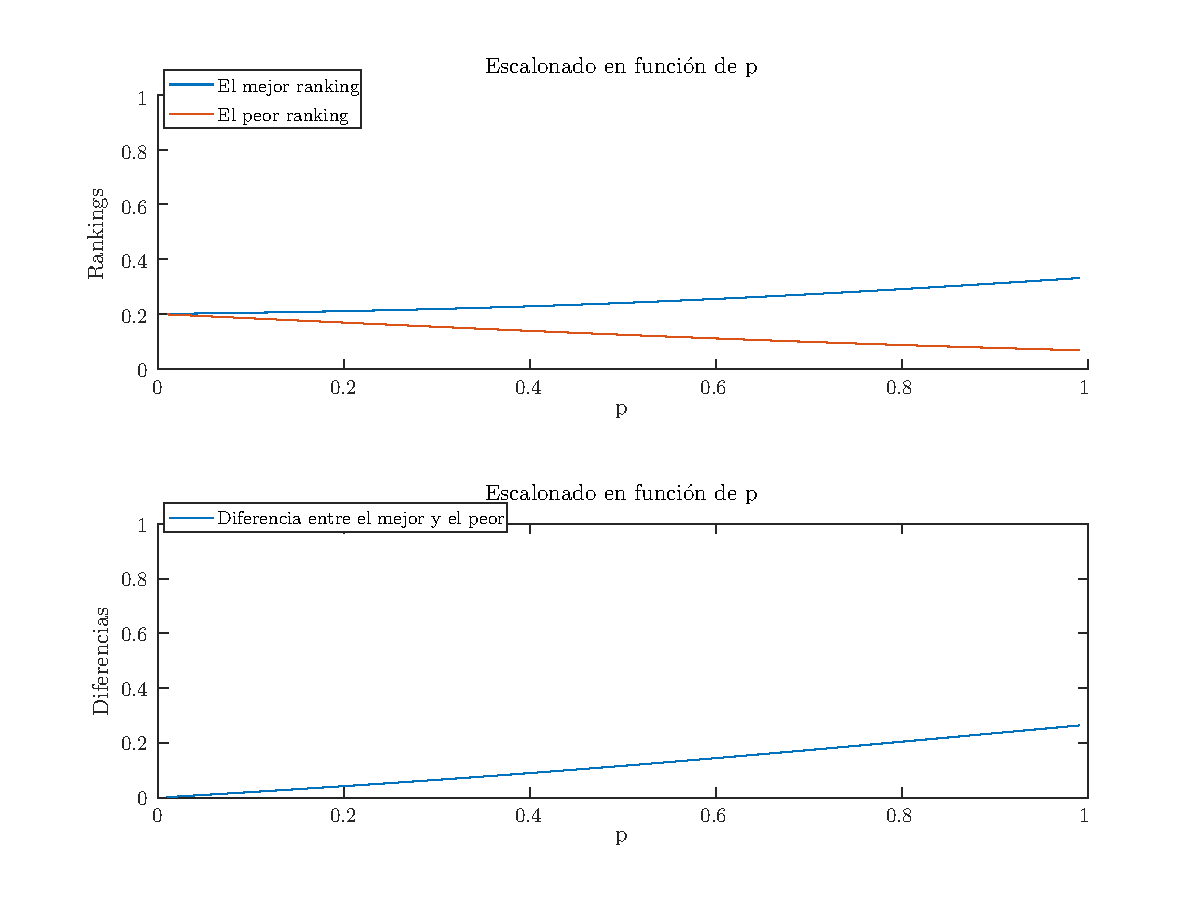
\includegraphics[ height=10cm, width=12cm]{../experimentacion/cualitativo/escalonado/escalonado_distintos_p}
\caption{variación de mejor y peor ranking con respecto a p}
\end{figure}

\subsubsection{Roba éxito}
Se calcula el Page Rank con $p = 0.65$.

\begin{figure}[H]
\centering
\includegraphics[ height=10cm, width=13cm, trim=0 2cm 0 0,clip]{../experimentacion/cualitativo/roba_exito/roba_exito_rank}
\caption{ranking con $p = 0.65$}
\end{figure}

\clearpage
\section{Discusión}
%Se incluir´a aqu´ı un an´alisis de los resultados obtenidos en la secci´on anterior (se analizar´a
%su validez, coherencia, etc.). Deben analizarse como m´ınimo los ´ıtems pedidos en el
%enunciado. No es aceptable decir que “los resultados fueron los esperados”, sin hacer
%clara referencia a la teor´ıa a la cual se ajustan. Adem´as, se deben mencionar los resultados
%interesantes y los casos “patol´ogicos” encontrados.

% \subsection{Experimentación sobre predicados teóricos}
% \subsubsection{El valor de $p$ y el error del sistema}
% En la Figura 1 se puede observar claramente que a medida que $p$ crece, el error del sistema aumenta.
% De todas formas, si bien el valor de $p$ afecta la precisión de la solución, nuestro algoritmo se sigue comportando bien y 
% dentro de los parámetros aceptables en todo el espectro de $p$, ya que incluso con un $p$ cercano a uno, el error sigue en el 
% \'orden de $10^{-17}$.

\subsection{Experimentación con estructuras de datos}
Como vemos en las Figuras 1 y 2, el vector resulta mejor en cuanto a tiempos de ejecución. Dicha estructura tiene ciertas ventajas, como el uso eficiente de la memoria cache y su simplicidad en el uso de la memoria (por ejemplo, no requiere pedir y liberar memoria tan frecuentemente como el mapa).


\subsection{Experimentación cuantitativa}
\subsubsection{Aproximación de la solución}
Como vemos en la Tabla 1, nuestro programa hace una buena aproximación a la solución, siendo perfecta en el caso trivial. En los tests más simples (sin links y completo), se ve que la implementación se encuentra con pocos problemas, teniendo un error del orden de $10^{-17}$. Con tests más complejos, este error aumenta, pero incluso en los tests intensivos de 15 y 30 segundos se comporta dentro de lo esperable con errores del orden de $10^{-7}$.

\subsubsection{Error absoluto con respecto a los tests de la cátedra}
En la Tabla 2 podemos ver que nuestra implementación da resultados iguales a los de la cátedra en la mayoría de los casos. La única diferencia se encuentra en los tests más intensivos (de 15 y 30 segundos), donde se encuentra una pequeña discrepancia del orden de $10^{-7}$.


\subsection{Experimentación sobre distintas implementaciones}
\subsubsection{Error con distintos tipos de datos para almacenar punto flotante}
Al realizar la implementación, intentamos evitar distintas fuentes de imprecisión, una de ellas siendo los tipos de datos. Por esto, desde el inicio usamos \textit{long double}, que utiliza más memoria que los otros tipos de datos de punto flotante. Sin embargo, como se puede ver en la Tabla 3, no hay diferencia en el error al usar este tipo o \textit{double}. Lo que sí se puede diferenciar es entre estos dos y \textit{float}, teniendo éste errores ligeramente mayores, pero casi insignificantes.

\subsubsection{Error con distintos tipos de sumatoria}
Al probar distintos tipos de sumatorias para normalizar el resultado, esperábamos que este fuera una fuente de imprecisiones. Sin embargo, como se ve en la Tabla 4, tanto la suma más simple, como la que ordena antes los números, y la que usa el algoritmo de Kahan, dan un error exactamente igual, por lo que vemos que no es un paso crítico en la pérdida de precisión.


\subsection{Experimentación cualitativa sobre distintas estructuras de grafos}
\subsubsection{Malla}
En la Figura 3 podemos observar que independientemente de la probabilidad de saltar a otra página del conjunto, el ranking se mantiene igual en todas las páginas.
Siendo este un caso muy sencillo, podemos fácilmente ver que el algoritmo de Page Rank está haciendo lo que debe.
En este caso muy particular donde ninguna página es mejor que otra, es esperable y también es efectivamente el resultado, que el ranking sea el mismo para todas.

\subsubsection{Página popular}
Con la Figura 4 podemos notar que la Página 1, nuestra página popular, efectivamente se lleva el primer lugar en el Ranking de Page.
Más aún, todas las otras páginas tienen exactamente el mismo ranking, están todas empatadas en el segundo lugar.
Esto tiene mucho sentido, dado que la Página 1 recibe links de todas las páginas del conjunto, mientras todas las demas, no reciben links.
Sus puntajes dependen exclusivamente del valor de $p$. La única razon por la que sus valores no son despreciables, es que todavia tienen
probabilidad de ser visitadas espontaneamente gracias a que la probabilidad de elegir una página del sistema de forma aleatoria es $1 - p$, y para este experimento $p = 0.65$.\\

Con los gráficos de la Figura 5, se puede observar que a medida que $p$ crece, el mejor ranking es aún mejor, y de la misma forma,
el peor ranking es aún peor. También se puede ver en el segundo gráfico que la diferencia entre ambos gráficos crece. Pero lo que resulta más importante para este experimento, es que cuando $p$ toma un valor muy cercano a 0, la diferencia entre el mejor ranking y el peor (o los peores, esperando que los 4 peores sean iguales como sucedió con $p = 0.65$) también toma un valor cercano a cero.
Con estos resultados podemos concluir que nuestra hipótesis es cierta. Esto se explicaría con que, si la probabilidad de saltar
a otra página del sistema es muy alta $(1 - p)$, entonces la probabilidad de caer en cualquier página tiende a ser equiprobable, y por lo tanto el ranking es (casi) un empate.

\subsubsection{Escalonado}
Como se puede ver en la Figura 6, el resultado fue el esperado. La página 5 es el final de la cadena, de cierta forma todos los links del sistema terminan eventualmente en esta página.
Por lo que era esperable que esta sea la página con mejor ranking. Más aún, la página 1 es el inicio de la cadena, ningún link la apunta, por lo cual también tiene
sentido que sea la página con peor ranking. \\

Sin embargo, si bien el orden de los rankings fue el predicho, esperábamos que los valores estén aún más inclinados al final de la cadena.\\

Con el resultado de este experimento en la Figura 7 podemos concluir que cuando $p$ toma un valor muy pequeño,
arruina el ranking del sistema. Ya que los valores del ranking resultan muy similares, implicando que existe una uniformidad en la probabilidad de caer en cualquier página.

\subsubsection{Roba éxito}
Tal como muestra la Figura 8, los resultados de este experimento fueron los esperados. La Página 1 es la más popular, seguida de la Página 2, y en tercer puesto con un cuádruple empate, el resto de las páginas.
Es un resultado muy satisfactorio, dado que demuestra este aspecto tan importante del algoritmo.

\clearpage
\section{Conclusiones}
%Esta secci´on debe contener las conclusiones generales del trabajo. Se deben mencionar
%las relaciones de la discusi´on sobre las que se tiene certeza, junto con comentarios
%y observaciones generales aplicables a todo el proceso. Mencionar tambi´en posibles
%extensiones a los m´etodos, experimentos que hayan quedado pendientes, etc.

Se nos pidió realizar un sistema de ranking de páginas web que utilice el algoritmo de page rank explicado en el enunciado del trabajo práctico.\\

Escribimos el algoritmo en C++ usando nuestra propia implementación de matriz rala para ahorrar espacio en memoria y tiempo al ejecutar el programa. Támbien utilizamos el algoritmo de eliminación gaussiana visto en clase para poder resolver el problema.\\

Pudimos resolver las pruebas planteadas por la catedra con mejor aproximación de la que se pedía y en un tiempo similar.\\

Igualmente quisimos realizar experimentos para encontrar posibles mejoras y poner a prueba nuestro programa. Decidimos por un lado, probar lo que aprendimos en las clases de laboratorio sobre precisión de datos y por otro ver si se cumple lo que el algoritmo de page rank propone.\\

En las clases de laboratorio vimos distintos tipos de representación de datos como float, double y long double. Quisimos experimentar sobre qué tipo de dato produce menos error en nuestro programa. Llegamos a la conclusión que si bien long double y double tienen un error parecido conviene usar double, ya que ocupa menos lugar en memoria.\\

También vimos distintas formas de sumar valores no enteros. Quisimos probar cual producía menos error en nuestro programa. Como mencionamos anteriormente, no encontramos ningún algoritmo que se destaque más que otro.\\

Por último hicimos experimentaciones sobre el algoritmo de page rank. Page rank propone que puede calcular la importancia de una página contando la cantidad de links y la cálidad de cada uno. Es decir, los links de páginas importantes valen más. Pudimos concluir que esto es cierto en el experimento roba éxito que planteamos. Además experimentamos como influye el modelo del navegante aleatorio en el proceso de obtener el page rank de una página. Siempre cuando p tiende a 0 todas las páginas tienen aproximadamente un mismo ranking. Luego el valor de p influye de manera distinta a cada sistema dependiendo de su estructura.
\clearpage
\section{Apéndices}
%En el ap´endice A se incluir´a el enunciado del TP. En el ap´endice B se incluir´an los
%c´odigos fuente de las funciones relevantes desde el punto de vista num´erico. Resultados
%que valga la pena mencionar en el trabajo pero que sean demasiado espec´ıficos para
%aparecer en el cuerpo principal del trabajo podr´an mencionarse en sucesivos ap´endices
%rotulados con las letras mayusculas del alfabeto romano. Por ejemplo: la demostraci´on
%de una propiedad que aplican para optimizar el algoritmo que programaron para resolver
%un problema.

\subsection{Apéndice A: Enunciado}
\includepdf[pages=-]{../tp1.pdf}

\subsection{Apéndice B: Código fuente relevante numéricamente}
Agregamos el código usado para resolver el sistema (método resolver de MatrizRala).
\begin{lstlisting}
vector<ld> MatrizRala::resolver(ll gamma) {
    vector<ld> b(this->filas.size(), gamma);

    // Eliminacion gaussiana
    for (unsigned int i = 0; i < this->filas.size() - 1; i++) {
        for (unsigned int j = i + 1; j < this->filas.size(); j++) {
            this->restarFila(i, j, b);
        }
    }

    // Sustituyo para atras
    vector<ld> x;
    x.push_back(b.back() / this->elem(this->filas.size() - 1, this->filas.size() - 1));
    for (int i = this->filas.size() - 2; i >= 0; i--) {
        ld sum = 0;

        for (unsigned int j = i + 1; j < this->filas.size(); j++) {
            sum += this->elem(i, j) * x[this->filas.size() - j - 1];
        }
        x.push_back((b[i] - sum) / this->elem(i, i));
    }

    reverse(x.begin(), x.end());
    this->normalizar(x);
    return x;
}
\end{lstlisting}

\subsection{Apéndice C: Demostración A e.d.d. $\Rightarrow A$ inversible}

Si $A=((a_{i,j})_{i,j\in [1,n]})$ es una matriz de diagonal estrictamente dominante, entonces A es inversible \\
\underline{Demostraci\'on:} \\
Por contrarrecíproco:  Supongamos que $A$ no es inversible, entonces su núcleo no se reduce a cero, existe entonces un vector: $X =	\begin{pmatrix}
							x_{1} \\
                            x_{2} \\
							\vdots \\
							x_{n} \\
						\end  {pmatrix}\not= 0 $ tal que  $AX = 0$. \newline
						\\
Entonces, se tiene que:
\begin{equation*}
\forall j \in [1,n], \displaystyle\sum_{\substack{i = 1}}^n a_{i,j} x_{j}= 0
\end{equation*}
 \newline
Como $X \not= 0$, existe $x_{k} \not= 0$ tal que
$| x_{k} |  = \max\{{ |x_{i}|, i \in [1,n] }\}$.\newline
Tenemos:  $-a_{k,k} x_{k} =  \displaystyle\sum_{\substack{i = 1\\i\neq k}}^n a_{i,k} x_{i}$ , de donde $|a_{k,k} x_{k}| \leq \displaystyle\sum_{\substack{i = 1\\i\neq k}}^n |a_{i,k} x_{i}| $,\newline
y como : $\forall i \in [1,n], \frac{\left|x_{i} \right|}{\left|x_{k}\right|} \leq 1 $ , \newline
se obtiene:
\begin{equation*}
\left| a_{k,k} \right| \leq \displaystyle\sum_{\substack{i = 1\\i\neq k}}^n |a_{i,k} |  \frac{\left|x_{i} \right|}{\left|x_{k}\right|} \leq \displaystyle\sum_{\substack{i = 1\\i\neq k}}^n |a_{i,k} |
\end{equation*}
Finalmente, $\left| a_{k,k} \right| \leq  \displaystyle\sum_{\substack{i = 1\\i\neq k}}^n |a_{i,k} |  $ , lo cual es absurdo por hip\'otesis, absurdo que provino de suponer que A era no inversible.

\clearpage
\section{Referencias}

\begin{itemize}
  \item C++ Docs - http://www.cplusplus.com/reference/
  \item Octave Docs - https://octave.org/doc
  \item Stack Overflow - https://stackoverflow.com/
  \item Herramienta web para graficar grafos - graphonline.ru/en/
\end{itemize}

\clearpage



\end{document}
